%!TEX encoding = UTF-8 Unicode
% http://tex.stackexchange.com/questions/9559/drawing-on-an-image-with-tikz
\documentclass[a4paper,11pt]{article}
\usepackage[utf8]{inputenc}
\usepackage{tikz}
%%%<
\usepackage{verbatim}
\usepackage[active,tightpage]{preview}
\PreviewEnvironment{tikzpicture}
\setlength\PreviewBorder{5pt}%
%%%>

\begin{comment}
:Title: Tikz picture on image

It was discussed here:
http://tex.stackexchange.com/questions/9559/drawing-on-an-image-with-tikz
\end{comment}

\begin{document}
\begin{tikzpicture}
    \node[anchor=south west,inner sep=0] (image) at (0,0) {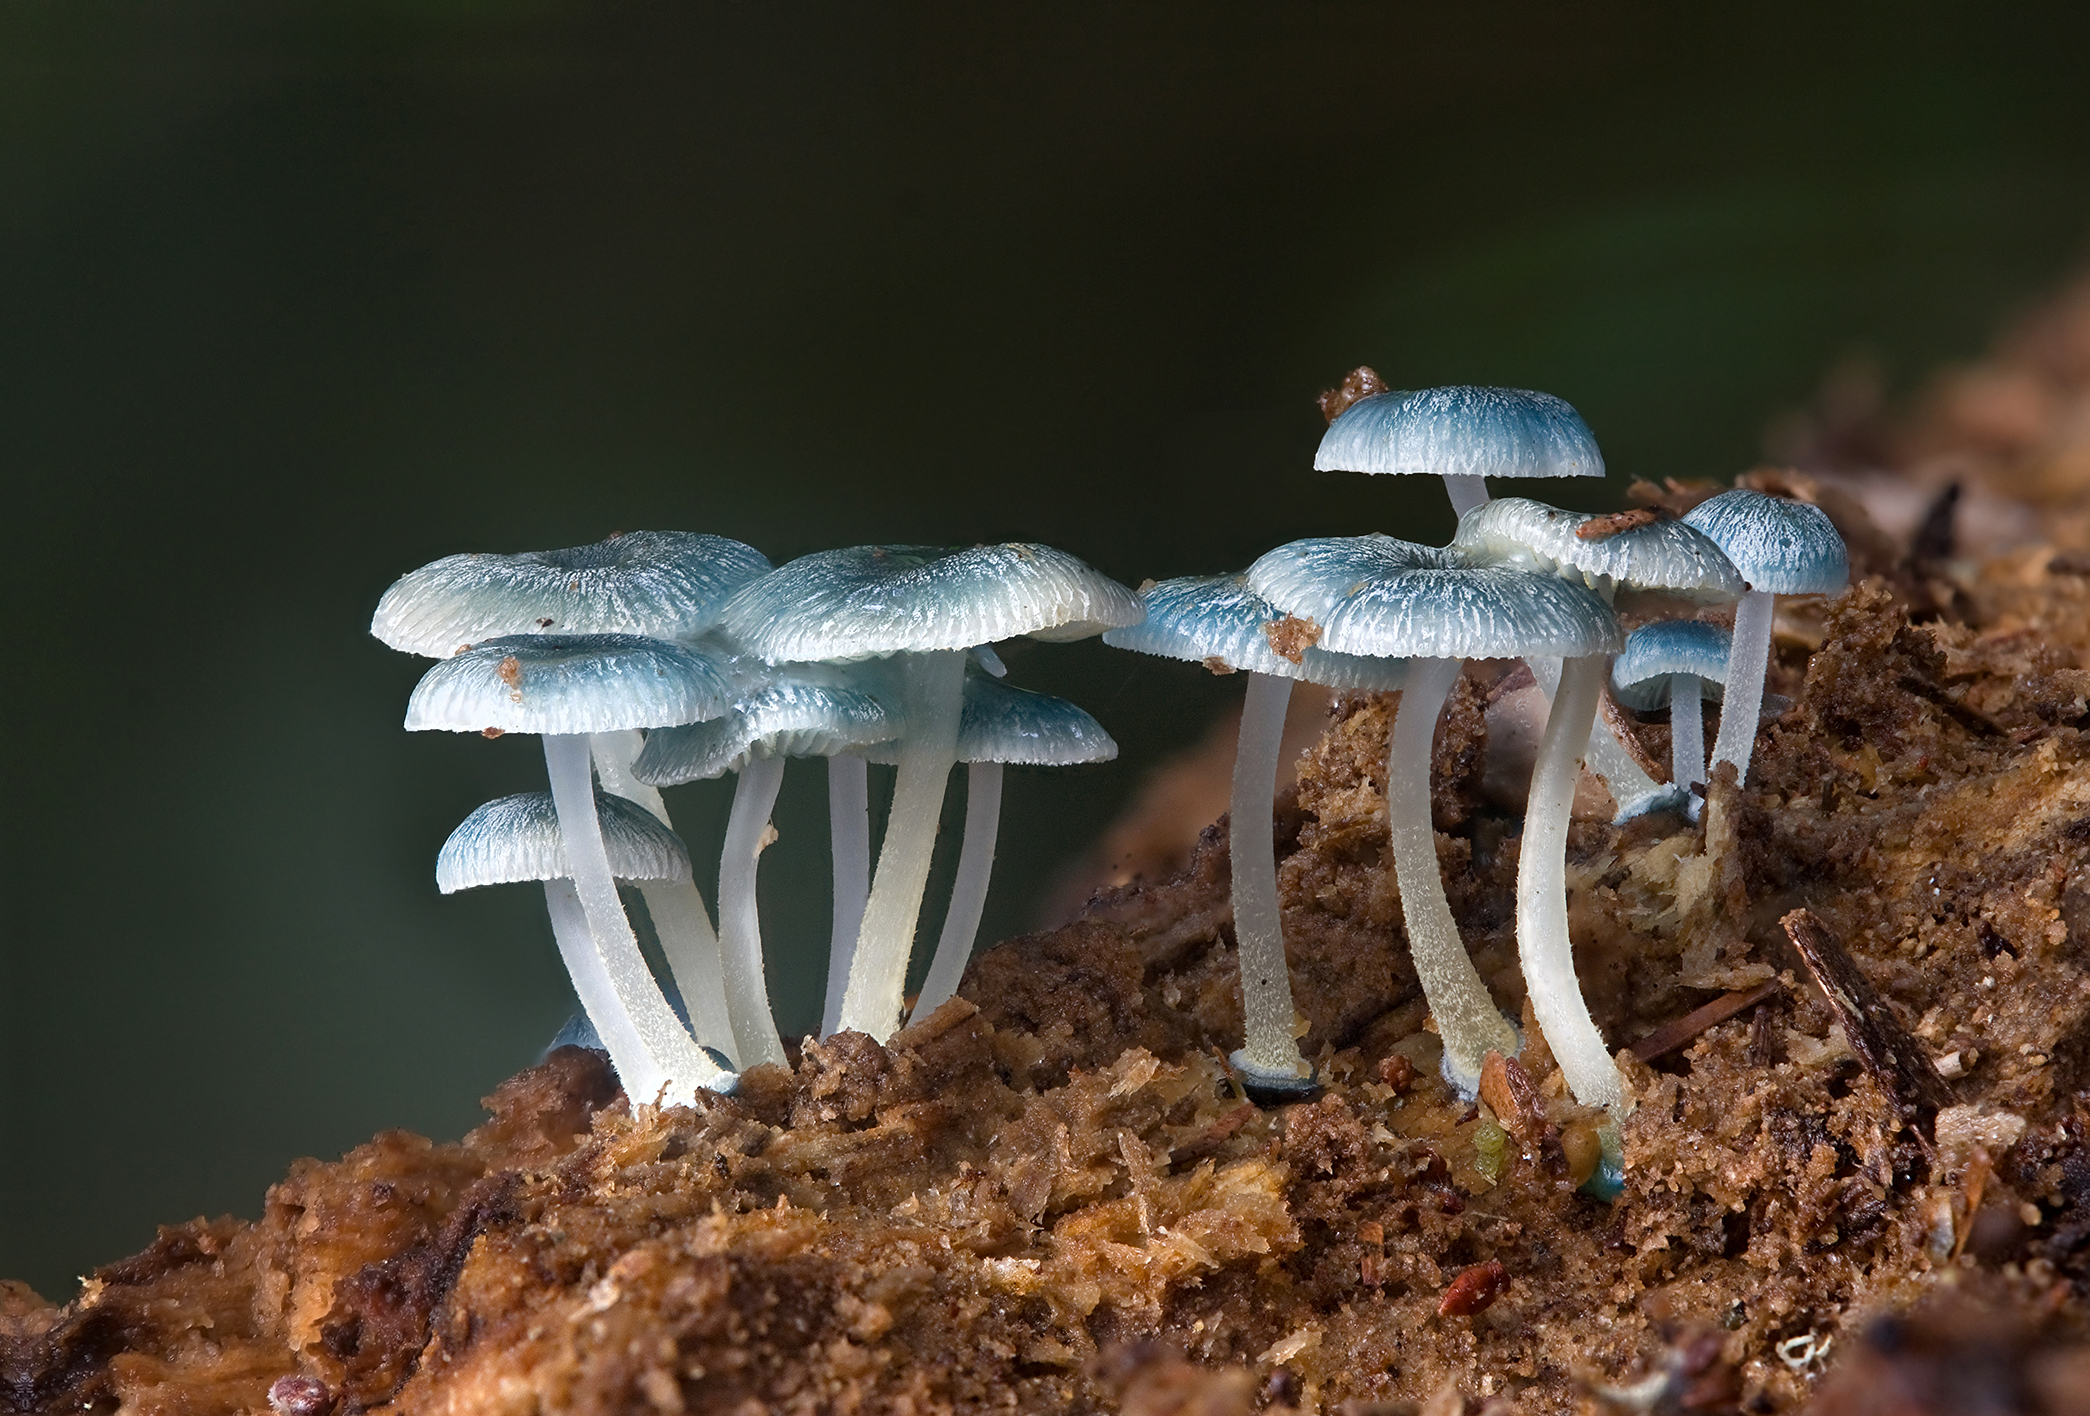
\includegraphics[width=0.9\textwidth]{Mycena_interrupta.jpg}};
    \begin{scope}[x={(image.south east)},y={(image.north west)}]
        \draw[red,ultra thick,rounded corners] (0.62,0.65) rectangle (0.78,0.75);
        \draw[help lines,xstep=.1,ystep=.1] (0,0) grid (1,1);
        \foreach \x in {0,1,...,9} { \node [anchor=north] at (\x/10,0) {0.\x}; }
        \foreach \y in {0,1,...,9} { \node [anchor=east] at (0,\y/10) {0.\y}; }
    \end{scope}
\end{tikzpicture}


\end{document} 
